The current situation is that 
\[
    M\times T^2 = V_- \times S_1 \bigcup_\Gamma V_+\times S_1
\] 
has a cobordism to $\Gamma \times S^2$.
The surgeries that turn $M\times T^2$ into $S^{2n+1}$ can be made disjoint from the dividing set, so it makes sense to talk about $\Gamma \subset S^{2n+1}$.
The full homology obstruction theorem states that any homology class in the dividing set $\Gamma$ that dies in a filling $W_\text{surg}$ of $S^{2n+1}$,
will also die in $V_\pm$.

For simplicity, in this thesis only a partial homology obstruction theorem will be proved, starting from a filling $W_\text{Bourgeois}$
of the Bourgeois manifold $M\times T^2$. What will be proved is that any homology class in the dividing set $\Gamma$ that dies in
$W_\text{Bourgeois}$ (all the more in $W$), will also die in $V_\pm$.

In order to make this more precise, define the inclusion maps
$i'\colon \Gamma \to \Gamma \times \{\operatorname{pt}\} \subset \Gamma \times S^2$ where $\operatorname{pt}$ is a point on the equator of $S^2$
and $i$ as the composition of $i'$ with the inclusion $\Gamma \times S^2 = \partial_+ C \hookrightarrow \partial W \hookrightarrow W$. 

Start with a cycle $z \in H_*(\Gamma, \mathbb Q)$ with $i_*(z) = 0 \in H_*(W, \mathbb{Q})$.
Consequently, there is a homology class $\sigma \in H_*(W, \mathbb Q)$ with boundary $i_*(z) = \partial \sigma$.
Any homology class in $\Gamma$ that dies in $W$ can be described in this way.
Intuitively, $\sigma$ can be pushed into $C_\pm$ in order to kill $z$ in $H_*(C_\pm, \mathbb{Q}) = H_*(V_\pm, \mathbb{Q})$.

More precisely, consider the commutative diagram
\[
\begin{tikzcd}
    \Gamma \arrow[r, hook, "i'"] \arrow[rrrr, bend left, "i"] \arrow[rrrdd, hook, "f_\pm"]
        & \Gamma \times S^2  = \partial W  \arrow[r, "\operatorname{ev}_\partial^{-1}", "\sim" below]
        & \partial \overline{\mathcal M}_* \arrow[r, hook, "j"]
        & \overline{\mathcal M}_*          \arrow[r, "\operatorname{ev}"] \arrow[d, twoheadrightarrow, "\pi"] \arrow[dd, bend right, "\mathcal I_\pi^\pm" left]
        & W \\
    &&& \overline{\mathcal M} \arrow[d, "\mathcal{I}^\pm"]  &   \\
    &&& C_\pm \simeq V_\pm                                  &   
\end{tikzcd}
\]
where $j$ and $\pi$ are the obvious inclusion respectively forgetful maps.
Recall that $\operatorname{ev}_\partial$ is the evaluation map restricted to the boundary of the moduli space. 
As proved in the last section, this map is a diffeomorphism close to the boundary and in particular on the boundary.
$\mathcal{I}^\pm\colon \overline{\mathcal{M}} \to W_\pm$ is the intersection map defined in the last section.
Finally, choose $\mathcal I_\pi^\pm$ and $f_\pm$ such that the diagram commutes.

The obstruction theorem states that already $f_{\pm,*}(z) = 0 \in H_*(C_\pm = V_\pm, \mathbb{Q})$.

Consider the set preimage $\operatorname{ev}^{-1}(\sigma) \subset \overline{\mathcal M}_*$.
As the boundary $\partial \sigma$ is contained in $\partial W$, the evaluation map is a diffeomorphism
and a neighborhood of $\partial \sigma$ is preserved under taking the preimage.
Away from this neighborhood, a slight perturbation might be necessary to make the resulting set a cycle in $\overline{\mathcal M}_*$.
%How does this work?
Clearly, the resulting cycle $\tau$ has boundary $\partial \tau \cong b$ and $\partial \tau$ is contained in the boundary $\partial \overline{\mathcal M}_*$.

%As $\pi$ maps $\partial \overline{\mathcal M}_*$ to $\partial \overline{\mathcal M}$, $\pi_*(\partial \tau)$ is contained in $\partial \overline{\mathcal M}$.
The following equation holds:
\begin{align*}
    \partial I_{\pi,*}^\pm(\tau) &= I_{\pi,*}^\pm(\partial \tau)\\
    &= I_{\pi, *}^\pm(\operatorname{ev}_{\partial, *}^{-1}(\partial \sigma))\\
    &= I_{\pi, *}^\pm(\operatorname{ev}_\partial^{-1}(i_*(z)))\\
    &= I_{\pi, *}^\pm\left((j \circ \operatorname{ev}_\partial^{-1} \circ i')_*(z)\right)\\
    &= f^\pm(z)
\end{align*}

As a result, $\left[f^\pm(z)\right] = \left[\partial I_{\pi,*}^\pm(\tau)\right] = 0 \in H_*(C_\pm, \mathbb Q) = H_*(V_\pm, \mathbb Q)$.
For a sketch of the proof, see \cref{fig:obstruction_proof_sketch}.

\begin{figure}
    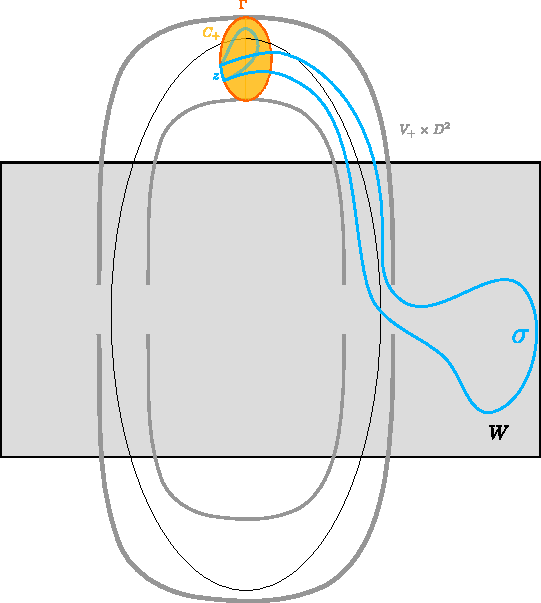
\includegraphics{../images/obstruction_proof_sketch.pdf}
    \caption{Sketch of $W$ with the two handles. The homology class $\sigma \in H_*(W)$ with boundary $z \in H_*(\Gamma)$ is pushed to $H_*(C_\pm)$.}
    \label{fig:obstruction_proof_sketch}
\end{figure}